\documentclass[aspectratio=169]{beamer}

%---------------------------
%       Beamer Cheat Sheet
%---------------------------
% https://www.cpt.univ-mrs.fr/~masson/latex/Beamer-appearance-cheat-sheet.pdf

%---------------------------
%       Set Theme and Colors
%---------------------------

\usetheme[width=.1\paperwidth]{Hannover}
% \setbeamertemplate{sidebar canvas right}[vertical shading][top=red,bottom=blue]

\definecolor{QESblue}{HTML}{8AD2ED}
\definecolor{QESdarkblue}{HTML}{187ca2}
\definecolor{QESlightblue}{HTML}{c4e8f6}

\setbeamercolor{sidebar}{bg=QESlightblue}
\setbeamercolor{titlelike}{fg=QESdarkblue}

\setbeamercolor{palette sidebar secondary}{fg=QESdarkblue}
\setbeamercolor{title in sidebar}{fg=QESdarkblue}
\setbeamercolor{author in sidebar}{fg=QESdarkblue}

\addtobeamertemplate{sidebar left}{}{\vfill \hspace{.006\paperwidth} 
\includegraphics[width=.08\paperwidth]{../../../logo.png} \vspace{.006\paperwidth} } 
% \addtobeamertemplate{sidebar left}{}{\vfill \hspace{.00001\paperwidth} 
\includegraphics[width=.093\paperwidth]{../../figures/qes-qr.png} \vspace{.003\paperwidth} } 

%---------------------------
%       No navigation symbols
%---------------------------
\setbeamertemplate{navigation symbols}{}

%---------------------------
%       Set Fonts
%---------------------------
\usepackage{helvet}
\renewcommand{\familydefault}{\sfdefault}
\usepackage{sansmathfonts}
\usepackage{upgreek}

\setbeamerfont{frametitle}{series=\bfseries, size=\Large}
\setbeamerfont{title in sidebar}{series=\bfseries, size=\small}
\setbeamertemplate{caption}{\it\raggedright\insertcaption\par}

%---------------------------
%       Math font packages
%---------------------------
\usepackage{dsfont, amsmath, amsthm, mathtools}
\usepackage{bbm, bm}
\usepackage[T1]{fontenc}
\usepackage[version=3]{mhchem}

%---------------------------
%       Figure packages
%---------------------------
\usepackage{graphicx}
\graphicspath{{../../figures}}

\usepackage{epstopdf}
\usepackage{color}

\setbeamerfont{caption}{size=\footnotesize}

\usepackage{subfigure}

%---------------------------
%       Manual placement packages
%---------------------------
\usepackage{tikz}
\usetikzlibrary{calc}

%---------------------------
%       Local Macros
%---------------------------

\newcommand{\manualpic}[4]{
    % inputs {filename}{figure options}{x offset}{y offset}
    \tikz[remember picture, overlay] \node[anchor=center] at ($(current page.center)+(#3,#4)$) {\includegraphics[#2]{#1}};
}

\newcommand{\manualtext}[3]{
    % inputs {text}{x offset}{y offset}
    \tikz[remember picture, overlay] \node[anchor=center] at ($(current page.center)+(#2,#3)$) {#1};
}

\newcommand{\manualtextleft}[3]{
    % inputs {text}{x offset}{y offset}
    \tikz[remember picture, overlay] \node[anchor=west] at ($(current page.center)+(#2,#3)$) {#1};
}

\newcommand{\manualtextright}[3]{
    % inputs {text}{x offset}{y offset}
    \tikz[remember picture, overlay] \node[anchor=east] at ($(current page.center)+(#2,#3)$) {#1};
}

\newcommand{\slidereference}[1]{
    \manualtextleft{\tiny #1}{-0.47\linewidth}{-0.47\textheight}
}

\newcommand{\dv}[2]{\frac{\mathrm{d}#1}{\mathrm{d}#2}}

\title{Ocean Carbon}
\author{4/5}

\begin{document}

\begin{frame}{The Carbonate Pump}
    
    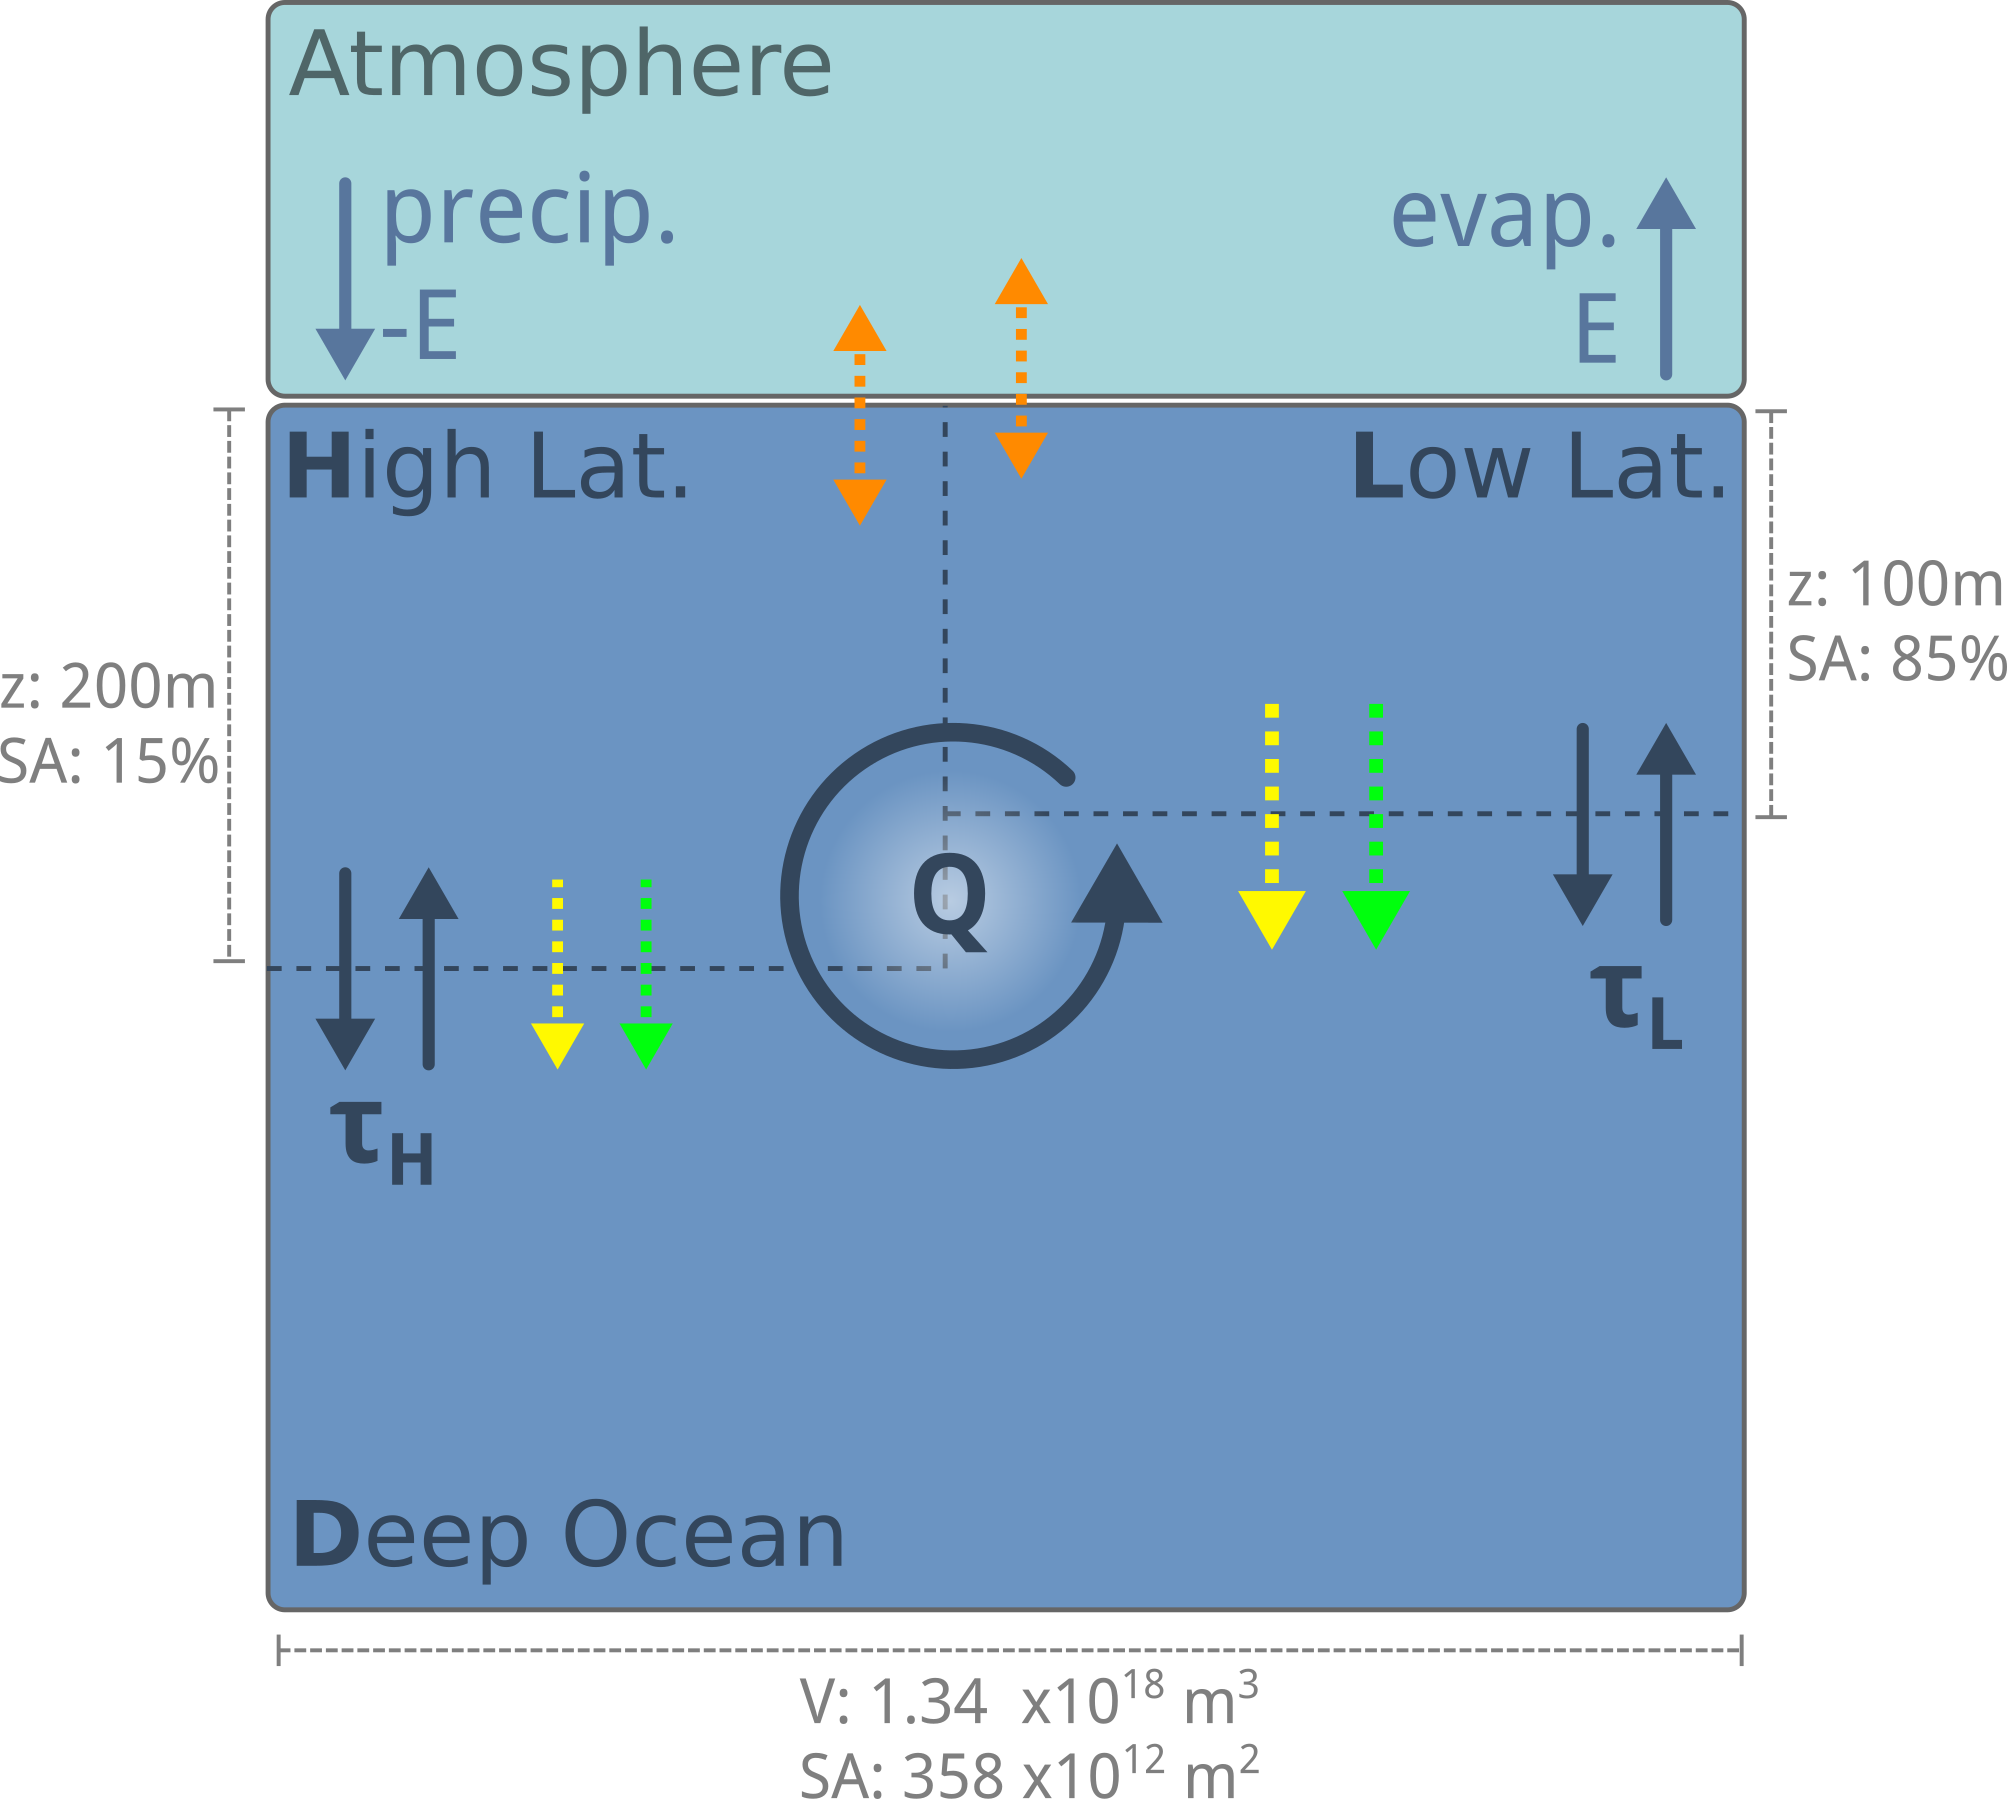
\includegraphics[width=\linewidth, totalheight=0.8\textheight, keepaspectratio]{ocean-3box-CO2-bio-calc.png}
        
\end{frame}

\section{Calcification}

\begin{frame}{Calcification}
    \centering

    \includegraphics<1|handout:1>[totalheight=0.7\textheight, keepaspectratio]{carbon-gastropod.jpg}
    \includegraphics<1|handout:1>[totalheight=0.7\textheight, keepaspectratio]{carbon-reef.jpg}

    \includegraphics<2|handout:2>[width=\linewidth, totalheight=0.8\textheight, keepaspectratio]{carbon-calcifiers.png}

\end{frame}

\begin{frame}{Production Patterns}
    \centering

    \includegraphics<1|handout:1>[width=\linewidth, totalheight=0.8\textheight, keepaspectratio]{carbon-caco3-export.png}

    \includegraphics<2|handout:0>[width=\linewidth, totalheight=0.8\textheight, keepaspectratio]{carbon-npp.png}

    \slidereference{Sarmiento \& Gruber (2006)}

\end{frame}

\begin{frame}{Active Biological Process}
    \centering

    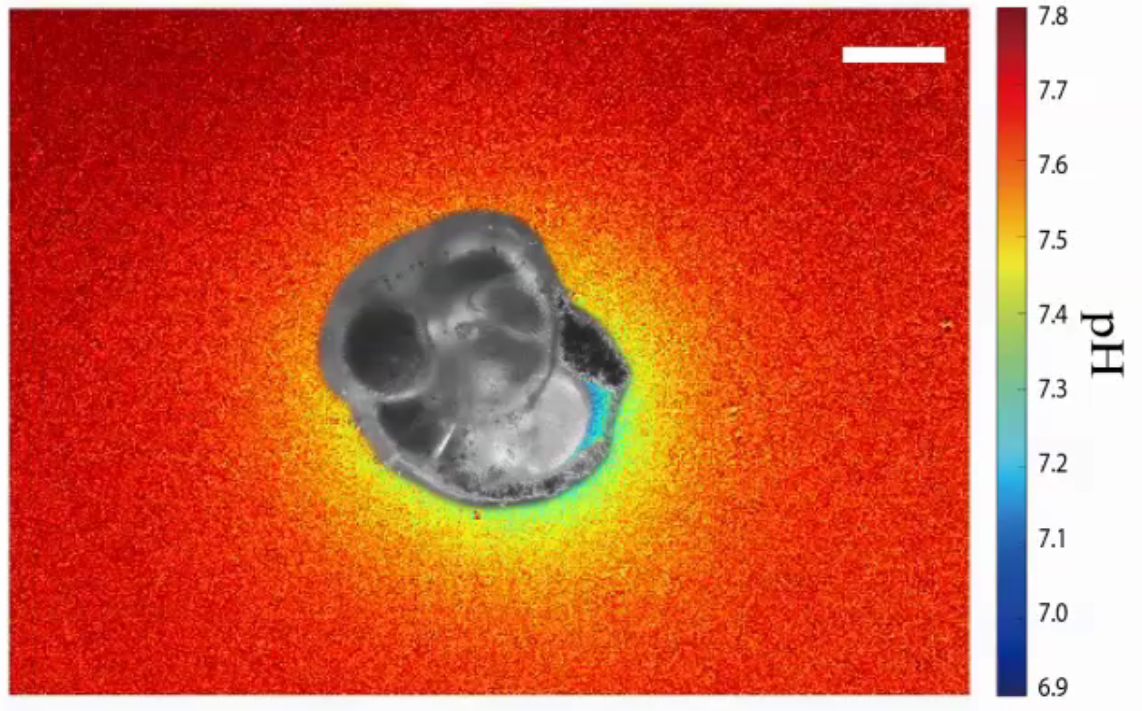
\includegraphics[totalheight=0.58\textheight, keepaspectratio]{carbon-foram-calc-external.png}
    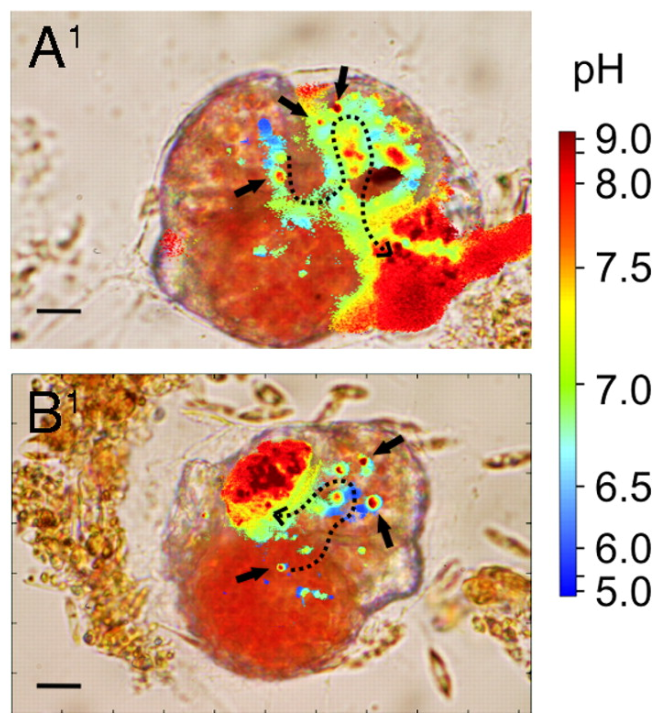
\includegraphics[totalheight=0.58\textheight, keepaspectratio]{carbon-foram-calc-internal.png}

    \slidereference{Toyofuku et al. (2017); De Nooijer et al. (2009)}

\end{frame}

\section{Chemistry}

\begin{frame}{Calcification}

    \centering

    $$
    \ce{CaCO3} \xrightleftharpoons[dissolution]{calcification} \ce{Ca^{2+} + CO3^{2-}}
    $$

    \onslide<2|handout:0>{
        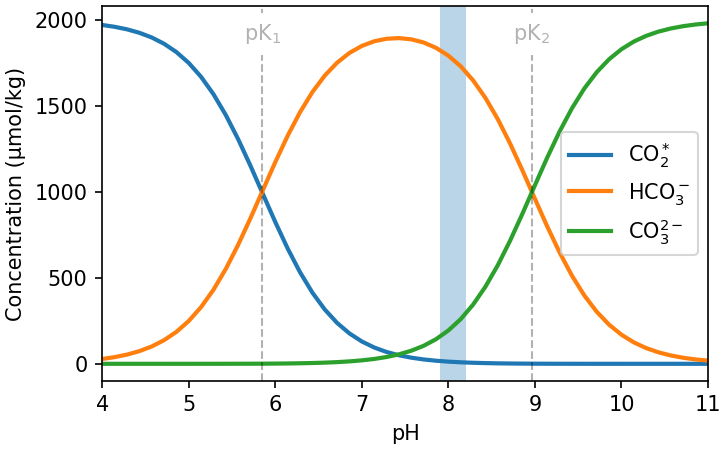
\includegraphics[width=\linewidth, totalheight=0.6\textheight, keepaspectratio]{carbon-bjerrum.png}
    }

\end{frame}

\begin{frame}{\ce{CO3^{2-}} Uptake?}

    \centering

    $$
    \ce{CaCO3} \xrightleftharpoons[dissolution]{calcification} \ce{Ca^{2+} + CO3^{2-}}
    $$

    \includegraphics<1|handout:1>[width=\linewidth, totalheight=0.6\textheight, keepaspectratio]{carbon-bjerrum-co3.png}

    \includegraphics<2|handout:2>[width=\linewidth, totalheight=0.6\textheight, keepaspectratio]{carbon-calc-co2-release.png}

\end{frame}

\begin{frame}<handout:0>{Calcification}

    \ce{CO3^{2-}} uptake by calcification...
    \begin{itemize}
        \item Removes DIC from the surface ocean.
        \item Shifts DIC speciation (removes TA from the surface ocean).
        \item Releases \ce{CO2} the atmosphere.
    \end{itemize}

    What happens at depth?
    
\end{frame}

\subsection{Saturation}

\begin{frame}{Saturation}

    \centering

    $$
    \ce{CaCO3} \xrightleftharpoons[]{K_{sp}} \ce{Ca^{2+} + CO3^{2-}}
    $$

    \onslide<2-|handout:1>{
        $$
        K_{sp} = (\ce{[Ca^{2+}]}\ce{[CO3^{2-}]})_{eq}
        $$
    }

    \onslide<3-|handout:1>{
        $$    
        \Omega = \frac{\ce{[Ca^{2+}]}\ce{[CO3^{2-}]}}{K_{sp}}
        $$

        Calcification when $\Omega > 1$; Dissolution when $\Omega < 1$.
    }

\end{frame}

\begin{frame}{Saturation}

    \centering

    \includegraphics<1|handout:1>[width=\linewidth, totalheight=0.8\textheight, keepaspectratio]{carbon-saturation-map.png}

\end{frame}

\subsection{Dissolution}

\begin{frame}{Pressure}
    \centering

    \includegraphics<1|handout:0>[width=\linewidth, totalheight=0.8\textheight, keepaspectratio]{carbon-CO3-sat.0.png}

    \includegraphics<2|handout:0>[width=\linewidth, totalheight=0.8\textheight, keepaspectratio]{carbon-CO3-sat.1.png}

    \includegraphics<3|handout:0>[width=\linewidth, totalheight=0.8\textheight, keepaspectratio]{carbon-CO3-sat.2.png}

    \includegraphics<4|handout:0>[width=\linewidth, totalheight=0.8\textheight, keepaspectratio]{carbon-CO3-sat.3.png}

    \includegraphics<5|handout:1>[width=\linewidth, totalheight=0.8\textheight, keepaspectratio]{carbon-CO3-sat.4.png}


\end{frame}

\begin{frame}{Pressure + Biological Pump}
    \centering

    \includegraphics<1|handout:1>[width=\linewidth, totalheight=0.8\textheight, keepaspectratio]{carbon-CO3-sat-real.png}

\end{frame}

\begin{frame}{Export Patterns}

    \includegraphics<1|handout:1>[width=\linewidth, totalheight=0.8\textheight, keepaspectratio]{carbon-caco3-export.png}

    \includegraphics<2|handout:2>[width=\linewidth, totalheight=0.8\textheight, keepaspectratio]{carbon-caco3-preservation.png}

    \includegraphics<3|handout:3>[width=\linewidth, totalheight=0.8\textheight, keepaspectratio]{carbon-seabed-topography.png}

    \slidereference{Sarmiento \& Gruber (2006)}

\end{frame}

\section{Carbonate Pump}

\begin{frame}{The Carbonate Pump}

    \centering 

    Exports \ce{CO3^{2-}} from the surface ocean to the deep ocean.
    
    \bigskip
    Moves TA and DIC in a 2:1 ratio:

    \begin{align*}
        \mathrm{DIC} &= {\color{red}\mathrm{[CO_3^{2-}]}} + \mathrm{[HCO_3^-]} + \mathrm{[CO_2^*]} \\
        \mathrm{TA} &= {\color{red}\mathrm{2[CO_3^{2-}]}} + \mathrm{[HCO_3^-]} + [\dots] - \mathrm{[H^+]} \\    
    \end{align*}

    Changes both carbon concentration and \textit{speciation}.

\end{frame}

\begin{frame}{The Carbonate Pump}

    \centering
    \includegraphics<1|handout:0>[width=\linewidth, totalheight=0.8\textheight, keepaspectratio]{carbon-circ-9-biopump-full.png}

    \includegraphics<2|handout:1>[width=\linewidth, totalheight=0.8\textheight, keepaspectratio]{carbon-circ-10-carbpump-full.png}

\end{frame}

\begin{frame}{TA and DIC export}

    \centering 

    \includegraphics<1|handout:0>[width=\linewidth, totalheight=0.8\textheight, keepaspectratio]{carbon-DIC-TA-calc.0.png}

    \includegraphics<2|handout:0>[width=\linewidth, totalheight=0.8\textheight, keepaspectratio]{carbon-DIC-TA-calc.1.png}

    \includegraphics<3|handout:0>[width=\linewidth, totalheight=0.8\textheight, keepaspectratio]{carbon-DIC-TA-calc.2.png}

    \includegraphics<4|handout:1>[width=\linewidth, totalheight=0.8\textheight, keepaspectratio]{carbon-DIC-TA-calc.3.png}

\end{frame}


\subsection{Ballasting}

\begin{frame}{Ballasting the Biologcial Pump}
    \centering

    \slidereference{Omand et al. (2020)}

    \begin{columns}
        \begin{column}{0.3\linewidth}
            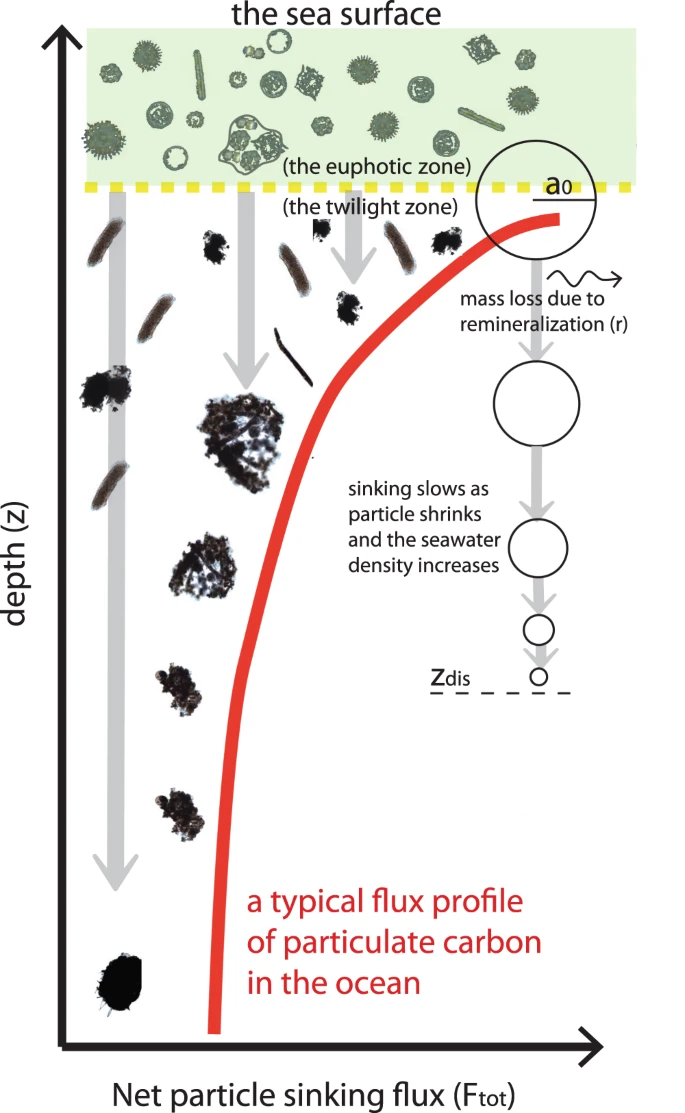
\includegraphics[width=\linewidth, totalheight=0.9\textheight, keepaspectratio]{carbon-particle-sinking.png}
        \end{column}
        \begin{column}{0.6\linewidth}
            \begin{itemize}
                \item Remineralisation relatively constant.
                \item Export efficiency depends on sinking speed.
                \item Sinking speed depends on density.
                \item Water $\sim 1025$, organic matter $1030-1500$, calcite $2710~\mathrm{kg~m^{-3}}$.
                \item Adding $\ce{CaCO3}$ increases particle density, sinking speed and biological pump efficiency?
            \end{itemize}
        \end{column}
    \end{columns}

\end{frame}

\subsection{Acidification}

\begin{frame}{Ocean Acidification}
    \centering

    \includegraphics<1|handout:0>[width=\linewidth, totalheight=0.8\textheight, keepaspectratio]{carbon-pCO2-pH.0.png}

    \includegraphics<2|handout:1>[width=\linewidth, totalheight=0.8\textheight, keepaspectratio]{carbon-pCO2-pH.1.png}
\end{frame}

\begin{frame}{Ocean Acidification - Feedbacks?}
    
    \textbf{Reduced calcification}
    \begin{itemize}
        \item Less \ce{CO2} released to atmosphere. \textbf{Negative Feedback}
        \item Reduced particle density, sinking speeds and biological pump efficiency. \textbf{Positive Feedback?}
    \end{itemize}
\end{frame}

\section{Modelling Carbonate Pump}

\begin{frame}{Modelling the Carbonate Pump}

    \begin{enumerate}
        \item Parameterise the export of \ce{[CO3^{2-}]} from the surface ocean as a function of biological productivity.
        \item Include the influence of \ce{[CO3^{2-}]} export on DIC and TA.
    \end{enumerate}

\end{frame}


\begin{frame}{1. Parameterise \ce{CacO3} Export}

    \ce{CaCO3} is produced by biological activity, so export will be tied to productivity via a factor:

    $$
    f_{calc} = \frac{DIC_{CaCO3}}{DIC_{organic}}
    $$

    The total export of \ce{[CO3^{2-}]} can then be calculated as a function of biological productivity:

    $$
    \dv{DIC_{calc, i}}{t} = \dv{\ce[CO3^{2-}]_{calc, i}}{t} = f_{calc} 106 \frac{V_i}{\tau^P_i} P_i
    $$

\end{frame}

\begin{frame}{2. Impact on DIC}

    \begin{align*}
        \dv{DIC_L}{t} &= \begin{bmatrix} \mathrm{transport} \\ \mathrm{CO_2~exch.} \\ \mathrm{bio.~pump.} \end{bmatrix} - f_{calc,L} 106 \frac{1}{\tau^P_L} P_L \\
        \dv{DIC_H}{t} &= \begin{bmatrix} \mathrm{transport} \\ \mathrm{CO_2~exch.} \\ \mathrm{bio.~pump.} \end{bmatrix} - f_{calc,H} 106 \frac{1}{\tau^P_H} P_H \\
        \dv{DIC_D}{t} &= \begin{bmatrix} \mathrm{transport} \\ \mathrm{bio.~pump.} \end{bmatrix} + \left(f_{calc,L} 106 \frac{V_L}{\tau^P_L} P_L + f_{calc,H} 106 \frac{V_L}{\tau^P_H} P_H \right) / V_D
    \end{align*}

\end{frame}

\begin{frame}{2. Impact on TA}

    \begin{align*}
        \dv{TA_L}{t} &= \begin{bmatrix} \mathrm{transport} \\ \mathrm{bio.~pump.} \end{bmatrix} - 2 f_{calc,L} 106 \frac{1}{\tau^P_L} P_L \\
        \dv{TA_H}{t} &= \begin{bmatrix} \mathrm{transport} \\ \mathrm{bio.~pump.} \end{bmatrix} - 2 f_{calc,H} 106 \frac{1}{\tau^P_H} \\
        \dv{TA_D}{t} &= \begin{bmatrix} \mathrm{transport} \\ \mathrm{bio.~pump.} \end{bmatrix} + \left( 2 f_{calc,L} 106 \frac{V_L}{\tau^P_L} P_L + 2 f_{calc,H} 106 \frac{V_L}{\tau^P_H} P_H \right) / V_D
    \end{align*}

\end{frame}


\begin{frame}{Impact of Carbonate Pump}
    \centering

    \only<1|handout:0>{Solubility Pump Only}
    \includegraphics<1|handout:0>[width=\linewidth, totalheight=0.8\textheight, keepaspectratio]{carbon-model-DIC-TA-pCO2.png}
    \only<1|handout:0>{$\mathrm{pCO_2} \sim 1300$}

    \only<2|handout:1>{Solubility + Biological Pumps}
    \includegraphics<2|handout:1>[width=\linewidth, totalheight=0.8\textheight, keepaspectratio]{carbon-model-DIC-TA-pCO2-bio.png}
    \only<2|handout:1>{$\mathrm{pCO_2} \sim 350$}
    
    \only<3|handout:2>{Solubility + Biological + Carbonate Pumps}
    \includegraphics<3|handout:2>[width=\linewidth, totalheight=0.8\textheight, keepaspectratio]{carbon-model-DIC-TA-pCO2-bio-carb.png}
    \only<3|handout:2>{$\mathrm{pCO_2} \sim 400$!}

\end{frame}

\end{document}


% \begin{frame}{TITLE}
% \end{frame}
